\documentclass[a4paper]{article}
\usepackage[x11names,svgnames]{xcolor}
\usepackage[T1]{fontenc}
\usepackage[utf8]{inputenc}
\usepackage[francais]{babel}
\usepackage{amsmath}
\usepackage{graphicx}
\usepackage{subfigure}
\usepackage[colorinlistoftodos]{todonotes}
\usepackage{array}
\usepackage{setspace}
\usepackage{fullpage}
\usepackage[justification=centering]{caption} % necessaire pour caption longue de plus d'une ligne.
\usepackage{hyperref} 
%\pdfcompresslevel=9 
\hypersetup{ 
     colorlinks=true, %colorise les liens 
     breaklinks=true, %permet le retour àˆ la ligne dans les liens trop longs 
     urlcolor= blue,  %couleur des hyperliens 
     linkcolor= Blue4, %couleur des liens internes crééŽs, 
}
\usepackage{listings}
\lstset{
language=python,
commentstyle=\textit,
basicstyle=\ttfamily\color{Black},
keywordstyle=\color{DarkRed},
commentstyle=\color{Blue3}\normalfont,
}
\newcommand{\cin}[1]{\lstinline{#1}}

% Francisation
\addto\captionsfrench{\renewcommand{\tablename}{{\scshape Tab.}}}

% Colonnes de largeur fixe
\newcolumntype{L}[1]{>{\raggedright\let\newline\\\arraybackslash\hspace{0pt}}m{#1}}
\newcolumntype{C}[1]{>{\centering\let\newline\\\arraybackslash\hspace{0pt}}m{#1}}
\newcolumntype{R}[1]{>{\raggedleft\let\newline\\\arraybackslash\hspace{0pt}}m{#1}}


\def\thesection{Question \arabic{section}}
\def\thesubsection{\alph{subsection}}

\onehalfspacing

% Bibliographie
\bibliographystyle{ieeetr}


\title{TP3 - IMN530}

\author{FOUQUET, Jérémie et MÉTHOT, Vincent}

\date{28 avril 2014}

\begin{document}
\maketitle

\section{IRM fonctionnelle}

Plusieurs outils d'analyse existent déjà pour traiter des données d'IRMf. Nous avons choisis de les utiliser directement plutôt que de les implémenter en python. Deux suites logicielles ont retenu notre intérêt (puisque nous les connaissons déjà), soit FSL [http://fsl.fmrib.ox.ac.uk/fsl/fslwiki/] et AFNI [http://afni.nimh.nih.gov/], qu'il faudra avoir installé pour faire fonctionner le script associé à ce numéro (Q1\_IRMf.sh).

\subsection{Étapes de reconstruction}

Il faut garder à l'esprit qu'à chaque étape de reconstruction, il est fortement conseillé d'inspecter visuellement les données. Dès leur réception, on a visuellement inspecté plusieurs tranches de \emph{fmri.nii} à tous les temps pour s'assurer que les artéfacts n'étaient pas trop important et que la correction de mouvement n'était pas nécessaire (voir Fig. \ref{fmri_anatomist}), comme mentionné dans la question. De plus, nous avons effectué une transformée de Fourier des séries temporelles (voir Fig. \ref{fmri_fft}).

\begin{figure}[h]
   \caption{\label{fmri_anatomist} Inspection visuelle de fmri.nii dans anatomist. On peut inspecter plusieurs tranches pour tous les points temporels à l'aide des deux curseurs à droite, comme dans un film.}
   \centering
   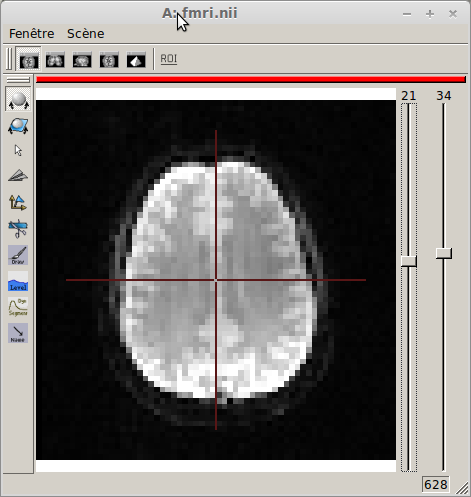
\includegraphics[width=\textwidth]{fmri_anatomist}
\end{figure}

\begin{figure}[h]
   \caption{\label{fmri_fft} Coupe sagitale de la transformée de Fourier de fmri.nii à chaque point. Une fréquence près de 0.02 Hz (la fréquence fondamentale du stimulus) est affichée dans AFNI. Les zones blanches peuvent être dues à de l'activation cérébrale mais aussi (et surtout) à un effet de bord relié à du mouvement.}
   \centering
   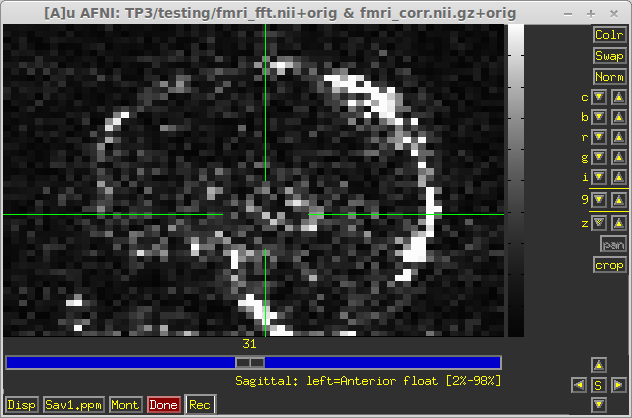
\includegraphics[width=\textwidth]{fmri_fft}
\end{figure}

Les étapes de reconstruction suivantes furent appliquées sur les données d'IRMf. Le résultat de chacune est illustrée sur la Fig. \ref{fmri_reconstruction}. On y voit sur la première ligne l'image originale (\ref{fmri_reconstruction}A - \emph{fmri.nii}) et les séries temporelles de quelques voxels voisins (\ref{fmri_reconstruction}B). Sur la deuxième ligne, il y a le résultat de la première étape de reconstruction ( \ref{fmri_reconstruction} A \& B \emph{fmri\_smooth.nii.gz}), c'est-à-dire l'image débruitée. Cette étape a pour but d'augmenter le rapport signal sur bruit par une convolution avec une gaussienne de FWHM = 6mm.
% Il y aurait avantage à utiliser un filtrage bilatéral, ou quelque chose de plus poussé...
La troisième ligne montre le résultat du filtrage temporel sur chaque voxel (\ref{fmri_reconstruction}E \emph{fmri\_low.nii.gz}). On voit par le fait même que la valeur moyenne de chaque voxel est fixée à 0, ne laissant que les variations temporelles. Comme du bruit et des artéfacts de nature physiologique se retrouvent aux hautes fréquences, nous avous décidé de couper les fréquences supérieures à 0.06 Hz (sachant que notre signal idéal à un fréquence fondamentale de 0.02 Hz) de chacune de nos séries temporelles (\ref{fmri_reconstruction}F).
La dernière étape de reconstruction consiste à calculer voxel par voxel une corrélation entre le signal idéal (contenu dans le fichier \emph{Data/ideal.txt}) et mesuré.  On en tire une carte de coefficients de corrélation entre -1 et 1 (\ref{fmri_reconstruction}F). On pourra ensuite seuiller cette carte pour obtenir un masque binaire des zones d'activations. La comparaison entre \ref{fmri_reconstruction}B et \ref{fmri_reconstruction}H montre l'effet du processus de reconstruction sur les données d'IRMf aurant au niveau spatial que temporel.

\begin{figure}[h]
   \caption{\label{fmri_reconstruction} A - Image originelle. B - Séries temporelles pour quelques voxels adjacents de l'image originelle. C - Image débruitée (convolution avec une gaussienne de FWHM = 6mm). D - Série temporelle débruitée. E - Image après passage d'une filtre passe-bas. La valeur moyenne (fréquence nulle) représentant l'information structurelle est perdue. F - Série temporelle de l'image filtrée. G - Corrélation point à point (seuillé à $\rho > 0.5$). H - Séries temporelles pour quelques voxels adjacents de l'image reconstruite. Position du point sélectionné: x = 22, y = 13, z = 24. Les séries temporelles rouge représentent le signal idée. Celles en noir représentent le signal mesuré/transformées.}
   \centering
   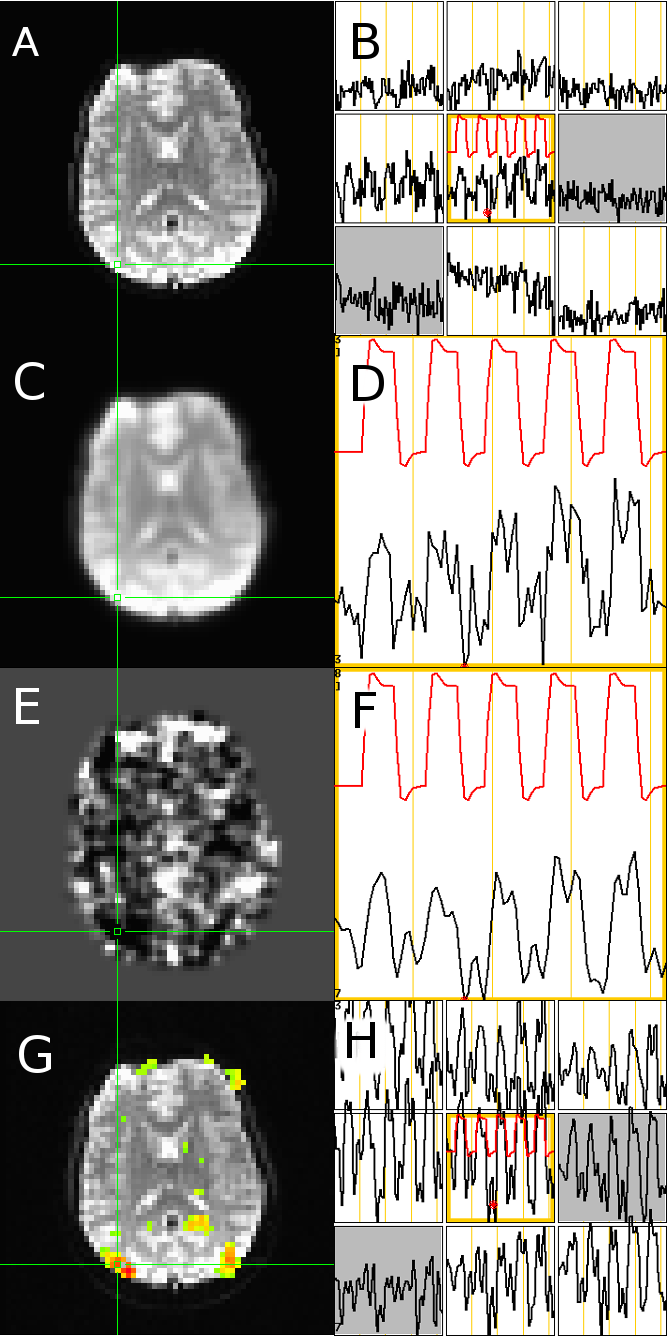
\includegraphics[height=0.85\textheight]{fmri_reconstruction}
\end{figure}


\subsection{Segmentation}

On a effectué la segmentation des zones d'activation à l'aide de l'outil graphique d'AFNI, de manière à trouver les paramètres idéaux en fonction des zones qu'on voulait voir activer. Puisque la tâche Roland est une tâche requérant des fonctions motrices, et mémoire et de vision, on s'attend à voir \og allumer \fg~ 6 zones reliées à ces activités. Les tâches motrices sont principalement localisées dans le cortex moteur (gyrus précentral). La mémoire est principalement localisée dans l'hippocampe. La vision est principalement localisée dans le cortex occipital. Nous nous sommes donc servis de nos connaissances anatomiques \emph{a priori} pour réaliser la segmentation et le regroupement des voxels activés (\emph{clustering}).

L'étape de segmentation dans le script \emph{Q1\_IRMf.sh} réalise l'opération de seuillage et de regroupement automatiquement, donnant 7 régions distinctes, dont chaqu'une est étiquetée avec une valeur diffénte:
	
\begin{enumerate}
    \item Lobe occipital droit (vision)
    \item Lobe occipital gauche (vision)
    \item Hippocampe gauche (mémoire)
    \item Hippocampe droit (mémoire)
    \item Gyrus précentral droite (mouvement)
    \item Région hors du cerveau (artéfact)
    \item Gyrus précentral gauche (mouvement)
\end{enumerate}

La méthode de segmentation utilisée consiste en un seuillage simple des valeurs de coefficient de corrélation (on ne garde que celles entre 0.5149 et 1), puis le \emph{clustering} de AFNI enlève les voxels n'étant pas regroupés. Plus précisément, les groupes comportant moins de 50 voxels voisins sont mis à zéro.

\subsection{Zones d'activation}



\section{IRM de diffusion}

\subsection{Estimation des tenseurs}
La fonction \lstinline{Q2_IRMd.tenseur} utilise la méthode de la pseudo-inverse pour effectuer le calcul des tenseurs. Elle peut prendre en entrée un masque qui indique pour quels voxels calculer les tenseurs. Sont également mis à 0 tous les éléments de tenseurs qui:
\begin{enumerate}
\item Correspondent à un signal à $b=0$ nul.
\item Prennent une valeur NaN ou Inf. 
\end{enumerate}
La fig. \ref{tenseurs_fiber} illustre les tenseurs que nous avons ainsi obtenus sur une carte de FA (calculée grâce à l'alogrithme présenté dans la section suivante).
\begin{figure}
\begin{center}
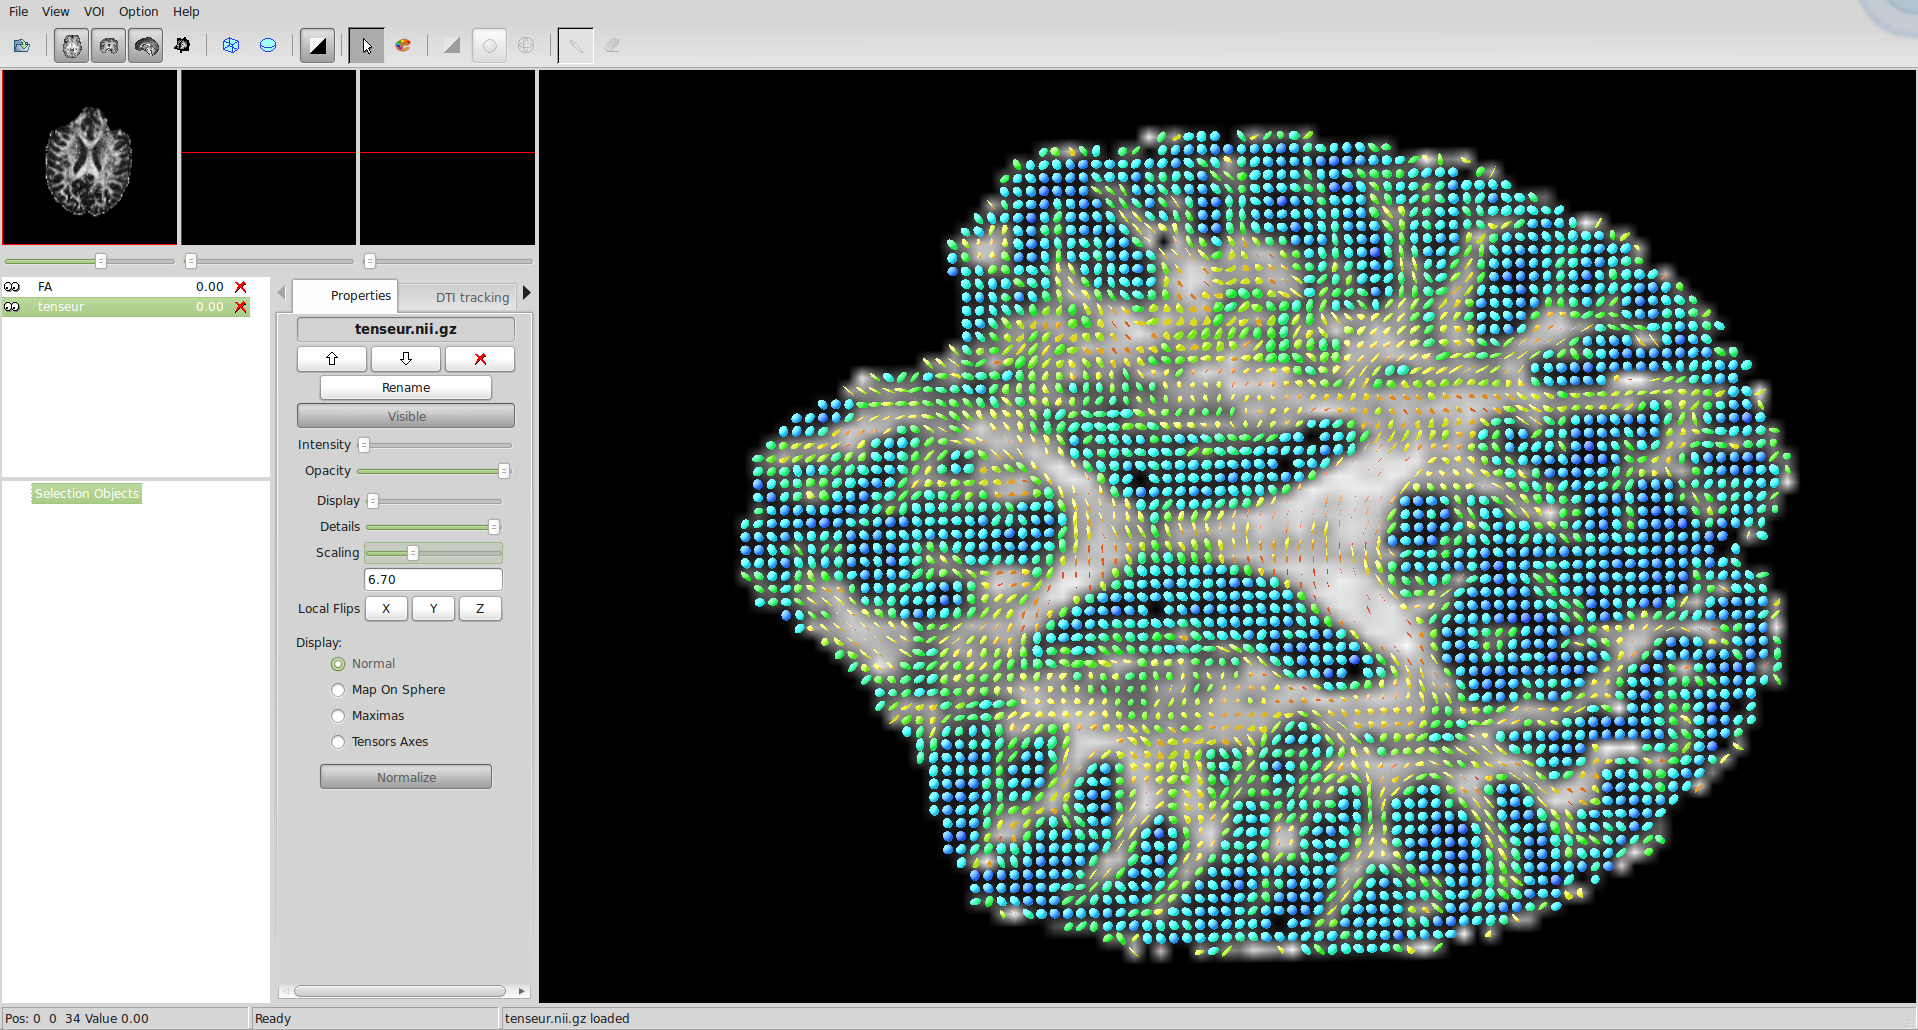
\includegraphics[scale=0.22]{tenseurs_fiber}
\caption{Illustration dans le Fibernavigator des tenseurs que nous avons obtenus grâce à la fonction \lstinline{Q2_IRMd.tenseur}. Les tenseurs sont superposés à la FA. À noter que seule une région identifiée comme étant le cerveau grâce à l'algorithme \lstinline{BET} de FSL est présentée. \label{tenseurs_fiber}}
\end{center}
\end{figure}

\subsection{FA et ADC}
La fonction \lstinline{Q2_IRMd.compAdcAndFa} calcule l'ADC et la FA à partir d'un champ de tenseur tel que calculé par la fonction \lstinline{Q2_IRMd.tenseur}. La fig. \ref{adc_fa} illustre pour certaines tranches l'ADC et la FA, respectivement. Les unités de l'ADC sont les mêmes que celles du coefficients de diffusion, soit $[longueur]^2/[temps]$, alors que la FA est sans unité.

\begin{figure}
\begin{center}
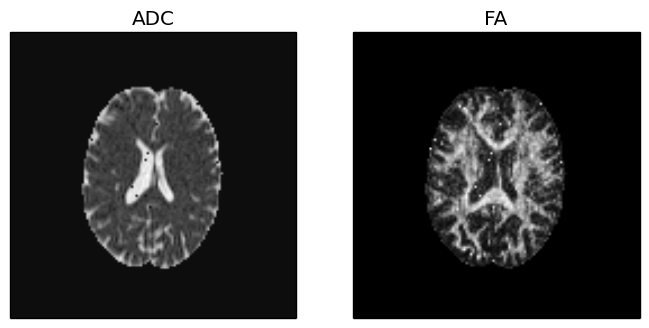
\includegraphics[scale=0.9]{adc_fa}
\caption{ADC et FA pour une tranche axiale du volume d'IRMd.\label{adc_fa}}
\end{center}
\end{figure}

\subsection{Tractographie}
La fonction \lstinline{Q2_IRMd.tracking} effectue une tractographie déterministe sur un champ de tenseurs. 

\paragraph{À quelle étape interpoler?} Lors de l'implémentation de la fonction, nous avons dû prendre une décision concernant la question suivante: \textit{quel champ doit être interpolé à chaque pas de la tractographie?} Nous avons considéré les options présentées dans le tab. \ref{tracto_interp}. Ces options ont toutes des avantages et des inconvénients: plus le nombres d'éléments à interpoler et le nombre de calculs à faire avant d'arriver à une direction de propagation sont grands, plus le temps de calcul total de l'algorithme sera grand. Cependant, comme on le voit dans le tab. \ref{tracto_interp}, la précision possible du résultat final diminue lorsque la vitesse de calcul augmente. Il en est ainsi car en général, ce qui permet d'interpoler moins d'éléments génère une perte d'information précédant l'interpolation (les transformées effectuées ne sont en effet pas réversibles). Les interpolations faites par la suite risquent donc d'être moins précises. Nous avons choisi une méthode qui semblait être un compromis entre temps de calcul et précision possible, soit \textbf{l'interpolation des tenseurs}. Nous n'avons cependant pas eu le temps de tester l'impact réel sur les temps de calcul et la précision des résultats.

\begin{table}
\begin{center}
\begin{tabular}{C{.3\textwidth}|C{.1\textwidth}|C{.1\textwidth}|C{.15\textwidth}|C{.15\textwidth}}
\textbf{Champ interpolé} & \textbf{Nb d'interp.} & \textbf{Nb de calculs} & \textbf{Vitesse de calcul}  & \textbf{Précision possible}\\ \hline
Mesures d'IRMd & 64 & 3 & \textcolor{red}{Basse} & \textcolor{green}{Haute} \\
Tenseurs avant (après) décomposition & 6 & 2 (1)& \textcolor{yellow}{Moyenne} & \textcolor{yellow}{Moyenne} \\
Direction du vecteur principal & 2 & 0 & \textcolor{green}{Haute} & \textcolor{red}{Basse}
\end{tabular}
\end{center}
\caption{Champs pouvant être interpolés lors d'un pas de tractographie, avec le nombre d'éléments devant être interpolés pour chacun d'entre eux (colonne 2) ainsi que le nombre de calculs manquants avant d'arriver à une direction de propagation (colonne 3). Plus ces nombres sont grands, plus le temps de calcul est grand. Cependant, en descendant dans les rangées du tableau, de l'information est également perdue avant l'interpolation. Ceci pourrait rendre l'interpolation moins précise. \label{tracto_interp}}
\end{table}

\paragraph{Méthode d'interpolation} La méthode d'interpolation a un impact crucial sur la vitesse de notre algorithme. Nous avons essayé les méthodes: plus proche voisin, linéaire et spline de degré $n$, avec $n$ allant de 2 à 5. Avec une méthode plus complexe que la méthode linéaire, l'interpolation devenait très visiblement le goulot d'étranglement de la vitesse de notre algorithme. Cependant, cela n'a pas causé d'amélioration apparente de la qualité de notre tractographie. Les autres résultats présentés dans ce rapport ont donc été obtenus avec avec la méthode d'interpolation linéaire. 

\paragraph{Résultats} La figure \ref{tracking} illustrent des fibres obtenues pour différents pas et différents seuil sur la FA, avec 10000 graines placées aléatoirement.

\begin{figure}
\begin{center}
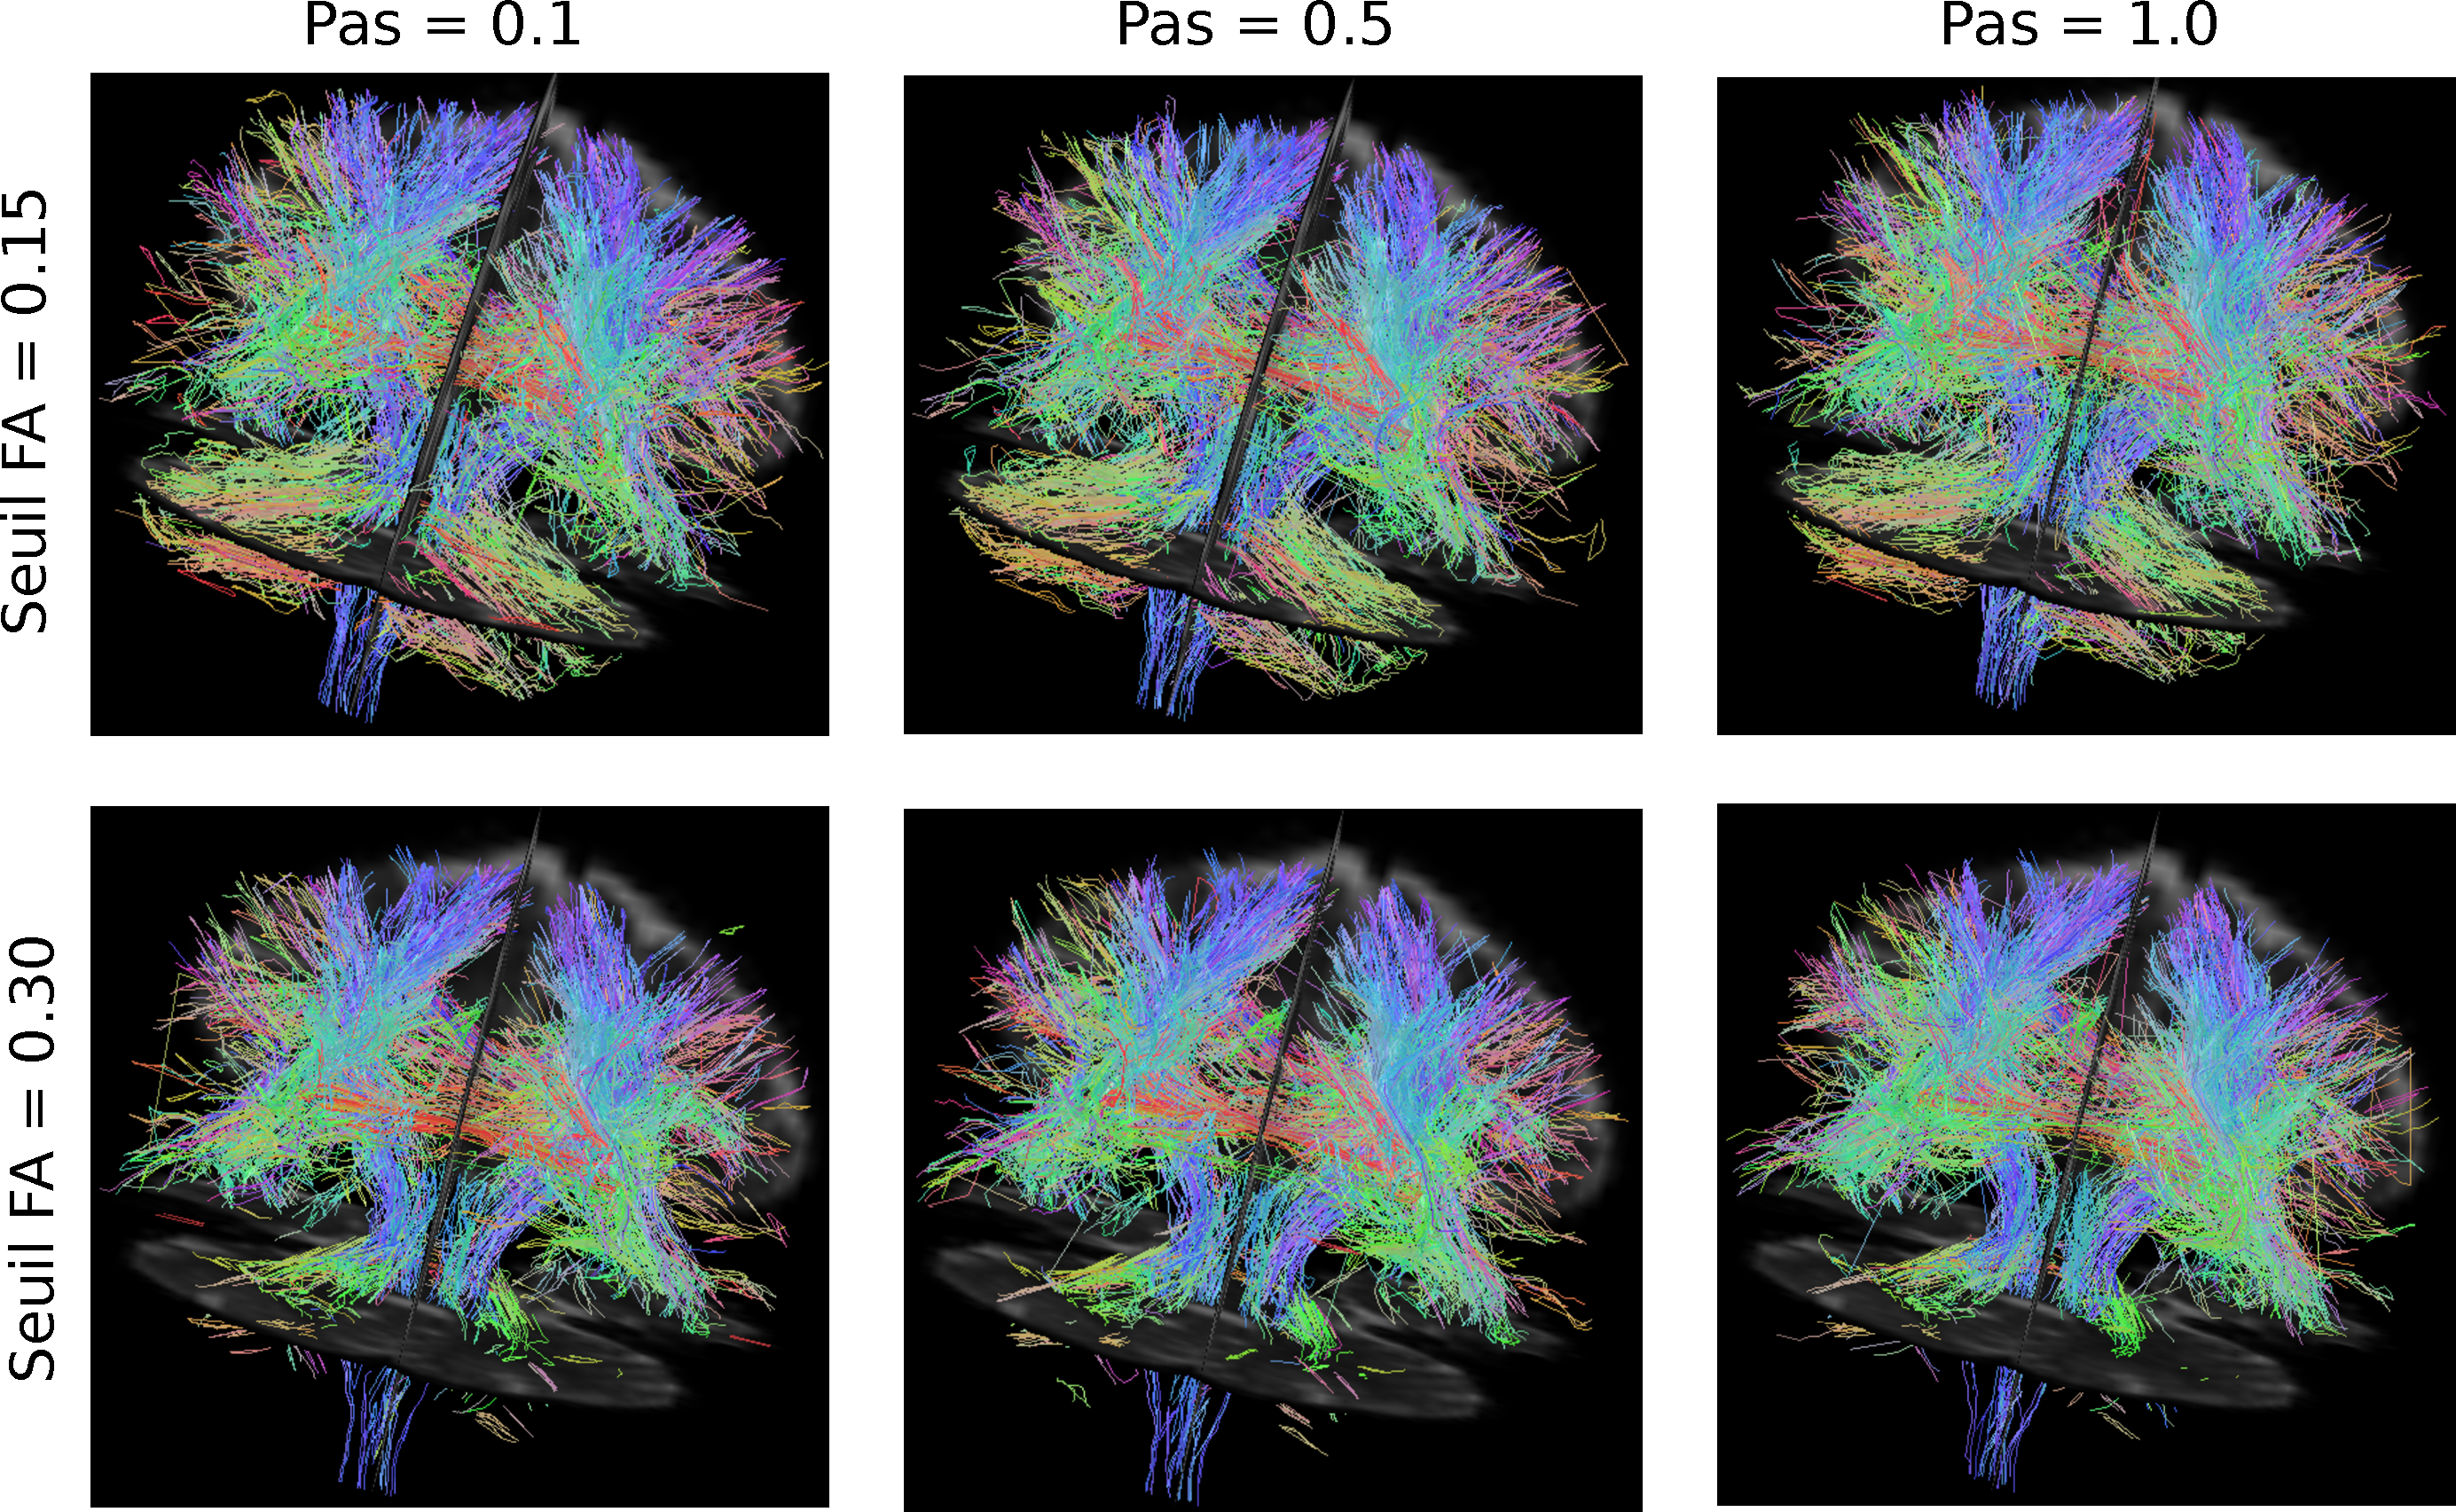
\includegraphics[scale=.3]{tracking}
\caption{Fibres obtenues avec 10000 graines placées aléatoirement pour différentes valeurs de pas et de seuil sur la FA visualisées dans le Fibernavigator et superposées à l'image à $b=0$. On voit bien une augmentation du nombre et de la longueur des fibres lorsque le seuil diminue. Cela est particulièrement visible dans le cervelet. Le pas ne semble pour sa part pas avoir une influence majeure sur l'apparence des fibres. \label{tracking}}
\end{center}
\end{figure}

\section{Fusion}

\subsection{Justification}

\subsection{Connectivité des zones fonctionnelles}

\section{Bonus}

\subsection{FA et ADC}

\subsection{Tractographie avec Dipy}


\end{document}